%%%%%%%%%%%%%%%%%%%%%%%%%%%%%%%%%%%%%%%%%%%%%%%%%%%%%%%%%%%%%%%%%%
%%%%%%%% ICML 2017 EXAMPLE LATEX SUBMISSION FILE %%%%%%%%%%%%%%%%%
%%%%%%%%%%%%%%%%%%%%%%%%%%%%%%%%%%%%%%%%%%%%%%%%%%%%%%%%%%%%%%%%%%

% Use the following line _only_ if you're still using LaTeX 2.09.
%\documentstyle[icml2017,epsf,natbib]{article}
% If you rely on Latex2e packages, like most moden people use this:
\documentclass{article}

% use Times
\usepackage{times}
% For figures
\usepackage{graphicx} % more modern
%\usepackage{epsfig} % less modern
\usepackage{subfigure} 

% For citations
\usepackage{natbib}

% For algorithms
\usepackage{algorithm}
\usepackage{algorithmic}

% As of 2011, we use the hyperref package to produce hyperlinks in the
% resulting PDF.  If this breaks your system, please commend out the
% following usepackage line and replace \usepackage{icml2017} with
% \usepackage[nohyperref]{icml2017} above.
\usepackage{hyperref}

% Packages hyperref and algorithmic misbehave sometimes.  We can fix
% this with the following command.
\newcommand{\theHalgorithm}{\arabic{algorithm}}

% Employ the following version of the ``usepackage'' statement for
% submitting the draft version of the paper for review.  This will set
% the note in the first column to ``Under review.  Do not distribute.''
\usepackage[accepted]{icml2017} 

% Employ this version of the ``usepackage'' statement after the paper has
% been accepted, when creating the final version.  This will set the
% note in the first column to ``Proceedings of the...''
%\usepackage[accepted]{icml2017}


% The \icmltitle you define below is probably too long as a header.
% Therefore, a short form for the running title is supplied here:
\icmltitlerunning{Submission and Formatting Instructions for ICML 2017}

\begin{document} 

\twocolumn[
\icmltitle{Effect of Signal Sparsity, Signal Density and Noise Level on Rotational Equivariant Features for Image Classification}

% It is OKAY to include author information, even for blind
% submissions: the style file will automatically remove it for you
% unless you've provided the [accepted] option to the icml2017
% package.

% list of affiliations. the first argument should be a (short)
% identifier you will use later to specify author affiliations
% Academic affiliations should list Department, University, City, Region, Country
% Industry affiliations should list Company, City, Region, Country

% you can specify symbols, otherwise they are numbered in order
% ideally, you should not use this facility. affiliations will be numbered
% in order of appearance and this is the preferred way.



\icmlsetsymbol{equal}{*}

\begin{icmlauthorlist}
\icmlauthor{Aliraza Punjani}{}
\icmlauthor{Apoorv Kulshreshtha}{}
\icmlauthor{Jamshed Shapoorjee}{}
\icmlauthor{Plaban Mohanty}{}
\end{icmlauthorlist}
\begin{center}
\{ amp2280, ak3963, js4962, pm2878 \}@columbia.edu
\end{center}
%\icmlaffiliation{to}{University of Torontoland, Torontoland, Canada}
%\icmlaffiliation{goo}{Googol ShallowMind, New London, Michigan, USA}
%\icmlaffiliation{ed}{University of Edenborrow, Edenborrow, United Kingdom}

\icmlcorrespondingauthor{Aliraza}{amp2280@columbia.edu}
\icmlcorrespondingauthor{Apoorv}{ak3963@columbia.edu}
\icmlcorrespondingauthor{Jamshed}{js4962@columbia.edu}
\icmlcorrespondingauthor{Plaban}{pm2878@columbia.edu}

% You may provide any keywords that you 
% find helpful for describing your paper; these are used to populate 
% the "keywords" metadata in the PDF but will not be shown in the document
\icmlkeywords{boring formatting information, machine learning, ICML}

\vskip 0.2in
]

% this must go after the closing bracket ] following \twocolumn[ ...

% This command actually creates the footnote in the first column
% listing the affiliations and the copyright notice.
% The command takes one argument, which is text to display at the start of the footnote.
% The \icmlEqualContribution command is standard text for equal contribution.
% Remove it (just {}) if you do not need this facility.

%\printAffiliationsAndNotice{}  % leave blank if no need to mention equal contribution
%\printAffiliationsAndNotice{\icmlEqualContribution} % otherwise use the standard text.
%\footnotetext{hi}





\begin{abstract} 
Current convolution methods for feature learning are already translation equivariant i.e. translation in input image produces a proportionate translation in feature maps. However, this is not true for rotational equivariance. A lot of recent research has been focussed on ensuring rotational equivariance for the same. Our research focusses on characterizing effect of different input image parameters, like sparsity, density and noise, on effectiveness of the learnt rotational equivariant features proposed in the recent work of Harmonic Convolutions. Feature maps learnt using Harmonic Convolutions exhibit equivariance to patch-wise translation and 360 degree rotation. These variant of normal convolutions use parameter-efficient and low computational complexity representation, thereby encoding complicated rotational equivariance within the network. In this paper, we show the effectiveness of rotational equivariance features for image classification as the sparsity, density and noise levels of the input image vary.

\end{abstract} 

\section{Introduction}
%\label{submission}

\section{Related Work}


\section{Problem Analysis}
Harmonic Convolutions hard bake 360 degree rotational equivariance into their feature representations by restricting the convolution filters to be from the circular harmonics family. In the following sections, we will discuss the properties of circular harmonics which help the network learn rotation equivariant features. To reiterate, rotational equivariance implies that a particular rotation in input image produces a proportionate rotation in feature maps.

\subsection{Circular Harmonics Equivariance}
We describe an image using polar co-ordinates r and $\phi$ as F(r , $\phi$). This can be understood better by looking at Figure \ref{fig:polarCoord}. Please note that this is just to depict the polar co-ordinates of a filter. In actual setting, the filter will be applied patch-wise to the image and therefore, a single image patch will be described using this method. \\
We will now show that there exists a filter $W_m$ such that the cross-correlation of F with $W_m$ yields a rotationally equivariant feature map. This condition is satisfied when $W_m$ is a circular harmonic of the form $W_m$ = R(r) $e^{i(m \phi + \beta)}$ for some m belonging to integers. Consider the rotation of original image by $\theta$ which leads to a new image F(r, $\phi - \theta$). The cross-correlation for the rotated image is

\vspace{-0.1cm}
\begin{center} 
[W * F(r, $\phi - \theta$)] = $\int$ W(r, $\phi$) F(r, $\phi - \theta$) dr d$\phi$ \\ \vspace{0.1cm}
$\hspace{80pt}$ = $\int$ W(r, $\phi$' + $\theta$ ) F(r, $\phi$') dr d$\phi$'
\end{center}
where $\phi$' = $\phi - \theta$. If we replace $W_m$ to be of the form R(r) $e^{i(m \phi + \beta)}$, then the integral transforms as:
\vspace{-0.1cm}
\begin{center} 
[W * F(r, $\phi - \theta$)] = $\int$ R(r) $e^{i(m (\phi' + \theta) + \beta)}$ F(r, $\phi$') dr d$\phi$' \\ \vspace{0.1cm}
$\hspace{75pt}$ = $e^{i m \theta}$ $\int$ R(r) $e^{i(m \phi' + \beta)}$ F(r, $\phi$') dr d$\phi$'
\end{center}
When rotation $\theta$ = 0, then $\phi$ = $\phi$'. Therefore, the above equation can be written as
\vspace{-0.1cm}
\begin{center} 
$\hspace{75pt}$ = $e^{i m \theta}$ $\int$ R(r) $e^{i(m \phi + \beta)}$ F(r, $\phi$) dr d$\phi$ \\ \vspace{0.1cm}
$\hspace{10pt}$ = $e^{i m \theta}$ [W * F(r, $\phi$)] 
\end{center}
Hence, we observe that the cross-correlation of the rotated signal F(r, $\phi - \theta$) with harmonic filter $W_m$ = R(r) $e^{i(m \phi + \beta)}$ is equal to the response at 0 rotation [W * F(r, $\phi$)] , multiplied by a complex phase shift $e^{i m \theta}$. Thus, we have shown that cross-correlation with $W_m$ yields a rotationally equivariant feature mapping when $W_m$ is a circular harmonic. 
\subsection{Chain rule for cross-correlation of circular harmonics}
In this section, we will show that the rotation order of a feature map, that we obtain after subsequent cross-correlations in each layer, is equal to the sum of the rotation orders of the filters in the chain.
Let us consider cross-correlation of a $\theta$ rotated image F(r, $\phi - \theta$)  with a filter $W_m$ and then followed by another cross-correlation with $W_n$. As shown previously, we write the response of first cross-correlation as  $e^{i m \theta}$[W * F(r, $\phi$)] . Then we can write the chain rule of harmonic cross-correlation as:
\vspace{-0.1cm}
\begin{center} 
$W_n$ * [$W_m$ * F(r, $\phi - \theta$)] = $W_n$ * $e^{i m \theta}$[$W_m$ * F(r, $\phi$)] \\ \vspace{0.1cm}
$\hspace{10pt}$ = $e^{i m \theta}$($W_n$ * [$W_m$ * F(r, $\phi$)])   \\ \vspace{0.1cm}
$\hspace{10pt}$ = $e^{i m \theta} e^{i n \theta}$ [ $W_n$ * [ $W_m$ * F]]  \\ \vspace{0.1cm}
$\hspace{10pt}$ = $e^{i (m + n) \theta} $ [ $W_n$ * [ $W_m$ * F]] 
\end{center}

Therefore, we see that chained cross-correlation results in a summation of the rotation orders of the individual filters $W_m$ and $W_n$.

\begin{figure}[t!]
  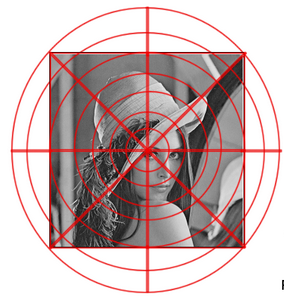
\includegraphics[width=\linewidth]{PolarImage.png}
  \caption{An image describing polar co-ordinates with image center as origin}
  \label{fig:polarCoord}
\end{figure}



\subsection{Circular harmonic filter architecture}

As we described in the previous sections, a Harmonic filter is defined as $W_m$ = R(r) $e^{i(m \phi + \beta)}$, so that it can capture the rotation equivariance while image classification. We also showed that whenever a test image is rotated, the cross-correlation of the rotated image with the learned filter, results in a product of  $e^{i m \theta}$ with [W * F(r, $\phi$)], where [W * F(r, $\phi$)] is the original non-rotated test image. Hence, the classifier is able to learn that any $e^{i m \theta}$ multiple of the original cross-correlation is the same image rotated by $\theta$, and thereby classify it correctly. Therefore, this clearly defined mapping helps achieve rotation equivariance of filters, which in turn leads to global rotation invariance of the network in predicting rotated images. This is the reason, the network is able to classify rotated images with equally good accuracy.
\begin{figure}[t!]
  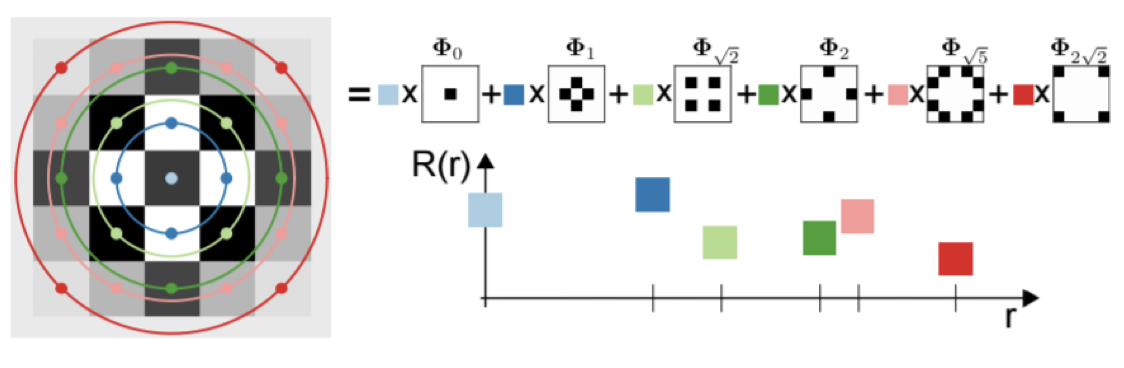
\includegraphics[width=\linewidth]{FilterArchitecture.png}
  \caption{Filter Architecture showing mapping of concentric harmonic filter profile to the cells of a square filter}
  \label{fig:FilterArch}
\end{figure}

We will now delve deeper into the architecture of a Harmonic filter.  The learnable parameters of a harmonic filter $W_m$ = R(r) $e^{i(m \phi + \beta)}$, are the radial profile R(r), which is a function of the radius r from the origin, and the per-filter phase offset $\beta$. For a n*n filter, the number of radial profile elements is equal to the number of rings of equal distance from the center of the filter. An example of this filter can be seen in Figure  \ref{fig:FilterArch}. This filter is a 5 * 5 filter with 6 rings of equal distance from the center of the filter. The smallest ring is just a single point. It is called a 5*5 filter because we are mapping the radial profile to the elements of a square filter with has length 5 and hence dimensions 5*5. And hence, this filter has 6 radial profile terms and 1 phase offset to learn. This is in contrast to a regular convolution filter which has 25 parameters to learn ( because of 5*5 dimension of the filter). 

Now, that we have explained the architecture of the harmonic filters, there is one very important characteristic to notice. Because we are learning a complete radial profile which depends only on the radius, the filter values for a particular radial profile are same, with only difference in sign. This can be perceived as an advantage as well as a disadvantage. Advantage because this kind of constraint enables the network to learn a rotation invariant classifier. And a disadvantage because the constraint doesn't let the network learn the filter freely during training , so that it can perform the best. In the next sections, we will see how this constraining of filters serves as an advantage as well as a disadvantage when looking at different applications.

To reiterate, till now the paper gives the reader a background of how Harmonic Networks work and how they are able to hard-bake rotation equivariance. More reference on this can be found in the paper [GIVE REFERENCE HERE]. From now on, we will discuss our main focus which describes how change in signal sparsity, signal density and noise level affects rotational equivariant features. 

\section{Parameters Affecting Rotational Equivariance}

\subsection{Noise}
Most of the image data used in real world applications are noisy in nature. One of the most important applications of image recognition and classification falls under the domain of supervision, intelligence and surveillance and despite the massive leaps in vision technology, the images captured by devices are quite noisy. While there has been good research in the fields of de-noising these images , the effort and computation required outweighs the performance of such methods. 
Hence, it is quite essential to analyze the effect of noise and its variations on harmonic filters to see if it still retains its accuracy and rotation equivariance . We also framed analytical conclusions based on the theory behind harmonic filters and performed experiments to confirm our understanding.

\textbf{Types of Noise :}

An image could have multiple variations of noise incorporated into it. Some of the most common ones are :

1.	Gaussian Noise : 

This is a form of additive noise added independently at each pixel. The added value is independent of signal intensity and is based on a gaussian distribution. One of the major reasons for this form of noise is the thermal noise (Johnson Nyquist Noise). This is one of the most common form of noise that arises due to low background illumination , increased temperature etc.

2.	Shot Noise :

This is a noise caused due to exposure fluctuations during the time the image is captured. It is caused different counts of photons sensed at a exposure level. It is dependent on the image intensity and is based on a Poisson distribution. As a result, apart from lower values of intensity its effects mimic Gaussian distribution

3.	Uniform Noise : 

It is caused by quantizing pixels of an image to discrete levels .the distribution of such a noise is uniform.

4.	Periodic Noise :

This noise appears as a periodic or iterating pattern over the image and is usually caused by electromagnetic interference while capturing the image.

\textbf{Analysis of effect of noise : }

For our analysis, let us assume Gaussian noise . As it is a form of additive noise that is independent of intensity , the variation is induced by the general std deviation of the gaussian distribution the noise is based on . Random noise values are added to the pixels from within the gaussian distribution. 

As we start off with lower values of std deviation , the variation in the values of noise added to the pixels are not significantly large. Hence the original image can still be retrieved from the noisy image as the added noise value is nearly equal with less variation across all the pixels. 

Considering our equation no (TBA), upon normalization, the harmonic filters are still able to get a multiple of the original cross correlation from the cross correlation of the noisy rotated image. The hard baked harmonic filters identify the corresponding pixel values  which although modified by a similar value throughout , are recognizable as their variation is less and hence they still retain their original pattern in the patch even after being scaled up (or down, depending on the noise added). Hence the harmonic filters perform almost as well with noise with low variance as they do without noise.

However, as the variance or std deviation of the gaussian distribution to which the noise belongs to increases , the variation of randomness in the addition of values to the pixels increases . As a result the pattern in the patch that we described earlier is lost i.e the change in pixel values are not constant and vary a lot. This makes it highly difficult for the harmonic filters to retrieve the cross correlation as a multiple of the original cross correlation. The F(r,phi) that we get here might be different from the original noiseless image .Hence it is difficult to classify the representation of the image. Although harmonic convolutions still preserve rotational equivariance, the original pattern of the image is altered and as a result the harmonic filters are not able to classify the image properly leading to lower accuracy.

This property makes the harmonic convolution exhibit similar traits as convolutional filters and hence the results reflect a similar pattern.

\textbf{Experimental Setup :}

To observe the variation in performance of the filters with noise, we chose to experiment with adding varying levels of Gaussian Noise. We used python libraries to introduce both noise and rotation in the images. To produce variation in noise levels, we kept the mean as 0 and increased the standard deviations or variance to observe the effects. 

To provide a basis of comparison for such results, we also ran a similar setup with convolutional neural networks . To further study only the effects of noise on harmonic filters and factoring out the rotational equivariance property , we also ran the experiments with non rotated noisy data on CNNs. The neural network architecture used for both the CNNs was VGG-16 .<Ref>
The entire experimental analysis was done on CIFAR-10 image dataset with 60k images 

\begin{figure}[t!]
  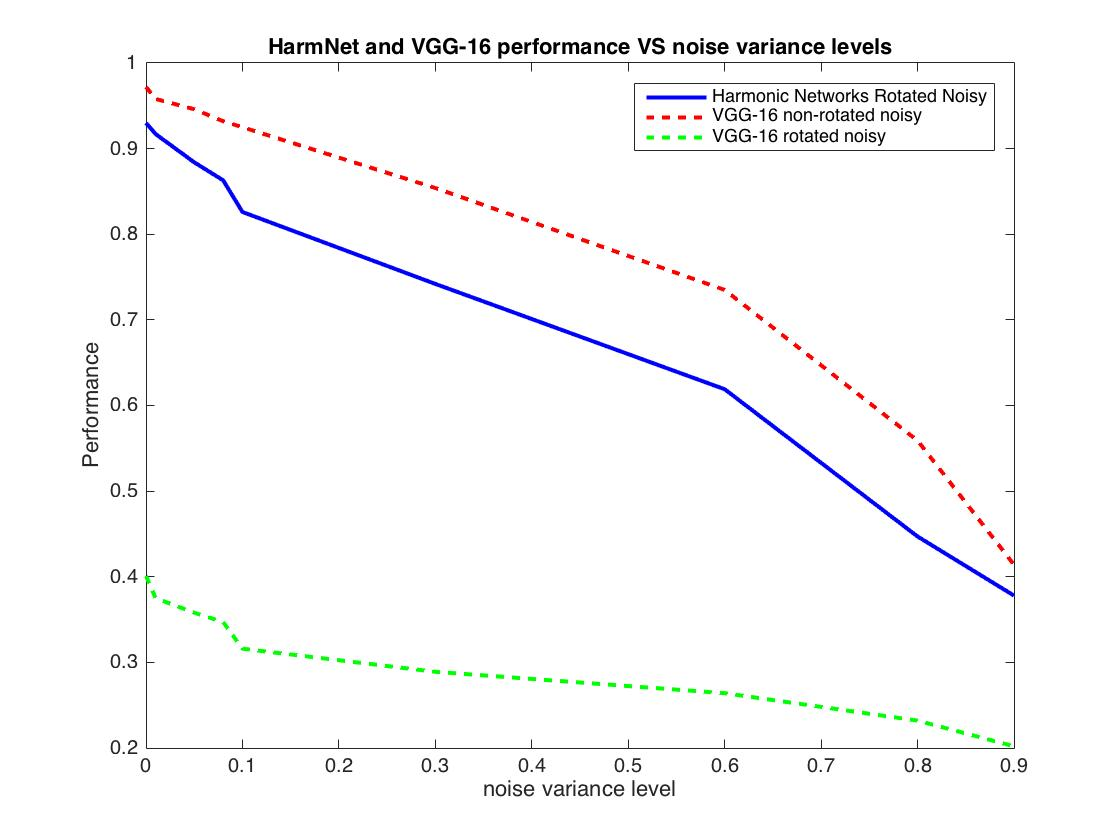
\includegraphics[width=\linewidth]{vggAndHarmVsNoise.jpg}
  \caption{Graph showing trend of accuracy with increase in noise}
  \label{fig:NoiseGraph}
\end{figure}
 
\textbf{Experimental Analysis :}

As can be observed from the graph in Fig 3 , the harmonic filters perform well in the lower values of variance in additive noise but steadily decrease as the variance increases .The same trend is observed in neural networks with non-rotated noisy images as well .An interesting point to observe is that the accuracy of harmonic filters is less by a near constant amount with respect to CNNs on non-rotated image across the entire graph. It has to be remembered that while the harmonic convolutions are on the rotated images, this CNN is on non-rotated images. The decreased performance is due to the restricted condition of the harmonic filters which learn parameters for rotation equivariance, however filters for CNN are free to learn and are unrestricted.
With same kind of data, both rotated and noisy, CNNs perform extremely poor in comparison to harmonic filters

\subsection{Sparsity}

Sparse representations of image data are widely used and recognized in the field of vision and classification experiments. Their increased popularity owing to their suitability as a regularizer for general inverse problems as well as their ease in supportability in high dimensional spaces have made them widely used in almost all image representation problems. The ease in storing and accessing sparse representations also make it highly convenient for their use. With current research showcasing increased performance in certain cases of classification with sparse representations , it is highly essential that we analyze its effect on the harmonic filters to observe the change in rotation equivariance properties.

\textbf{Ways to induce sparsity in images :}

Sparse approximation problem is a highly researched topic with efficient algorithms to solve this problem in place . We list some of the most commonly used algorithms :

1.	Projected Gradient Descent : 

This is similar to normal gradient descent where the gradient shows the direction for movement. Since we are looking for a sparse solution, the putative solutions are projected onto the sparse scaffold of k vectors.

2.	 LASSO :

This regression analysis method is widely used along with its multiple variations. It solves the L1 norm version of the sparse approximation method . Fused Lasso ,Group Lasso and other variations are used for generating sparsity.

3.	Proximal Methods :

Proximal methods including proximal gradient descent is also used for induced sparsity in images .With thresholding /hard thresholding , the sparsity induced by this method forms the basis for many classification experiments.

\textbf{Analysis of Sparsity on images :}

To understand the effect of sparsity, we need to refer to the hard baked filters that are applied on patches of data. These filters as explained in the section above are concentric filters applies on pixels that in turn produce rotation equivariance. This method relies on the pattern of pixels on which the filter is applied. Now as we induce sparsity, some or most of the pixels are reduced to 0. Now, even though the pixels might not be relevant for image classification , this hinders the basic property of the pattern in the patches that the harmonic filters rely on. Hence the hard baked filters which learn in a constrained manner are not able to produce rotation equivariant features. 

We can visualize this with reference to fig.  where the harmonic paths are applied on a patch. Now , if we decrease the values of pixels to 0 , the purpose of the harmonic filter is defeated as with some removed pixel values , the filters do not apply on the similar kind of images as they have been trained on. As a result, in terms of cross correlation , the cross correlation value of the rotated sparse image is not a multiple of the cross correlation of the original image. Hence , the classification isn’t accurate. 

As this adversely affects the filters, the increase in sparsity should cause rapid decrease in performance of the classifier. Now, it can be observed that since these constraints are not present in the normal CNN filters , this massive decrease in performance is not observed in the case of normal convolutions. The constrained filters which produce rotation equivariance are also the cause for the decrease in accuracy of classification for harmonic convolutions .

\textbf{Experimental setup:}
 
The setup is the same as the experiments with noise. The variation in sparsity is produced by Python libraries and the percentage of sparsity is increased to observe the effect. 
The image data is CIFAR-10 with 60k images.
Similar to experiments with noise, we have kept two standard observations for comparison – CNN with non-rotated sparse images and one with rotated sparse representations.

\begin{figure}[t!]
  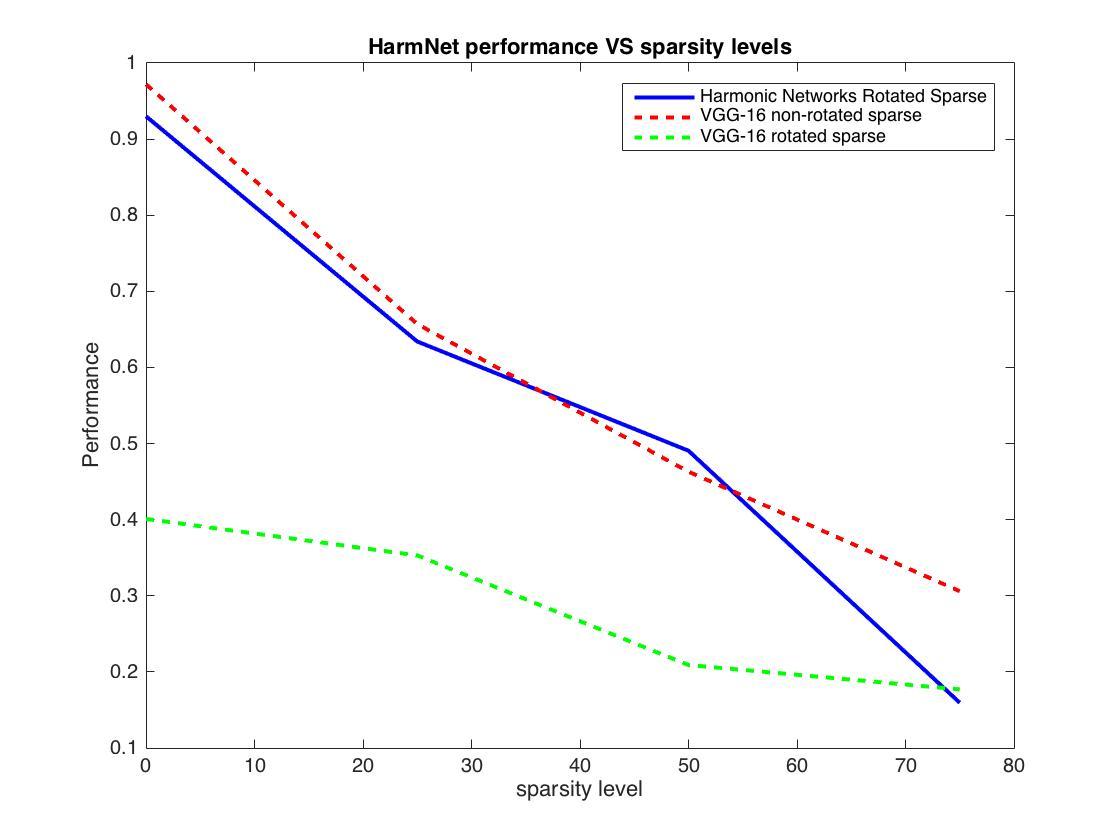
\includegraphics[width=\linewidth]{vggAndHarmVsSparse.jpg}
  \caption{Graph showing trend of sparsity with increase in noise}
  \label{fig:SparseGraph}
\end{figure}

\textbf{Experimental Results:}

As expected, there is a steep decline in the performance of the harmonic filters on increase in sparsity. With higher levels of sparsity, the filters perform poorly and lose their rotation equivariance property. Further on extremely high values of sparsity it is observed that due to the constrained filters in harmonic networks, the accuracy falls even below CNN on rotated ,sparse images. This stands as a testimony to the adverse effect of sparsity in harmonic networks.


\section{Conclusion}

\section{Future Work}

\section{References}

We will continue the ICML tradition in which the authors are given the
option of providing a short reaction to the initial reviews. These
reactions will be taken into account in the discussion among the
reviewers and area chairs.

\subsection{Submitting Final Camera-Ready Copy}

The final versions of papers accepted for publication should follow the
same format and naming convention as initial submissions, except of
course that the normal author information (names and affiliations)
should be given.  See Section~\ref{final author} for details of how to
format this.

The footnote, ``Preliminary work.  Under review by the International
Conference on Machine Learning (ICML).  Do not distribute.'' must be
modified to ``\textit{Proceedings of the
$\mathit{34}^{th}$ International Conference on Machine Learning},
Sydney, Australia, 2017.  JMLR: W\&CP. 
Copyright 2017 by the author(s).''

For those using the \textbf{\LaTeX} style file, simply change
$\mathtt{\backslash usepackage\{icml2017\}}$ to 

$$\mathtt{\backslash usepackage[accepted]\{icml2017\}}$$

\noindent
Authors using \textbf{Word} must edit the
footnote on the first page of the document themselves.

Camera-ready copies should have the title of the paper as running head
on each page except the first one.  The running title consists of a
single line centered above a horizontal rule which is $1$ point thick.
The running head should be centered, bold and in $9$ point type.  The
rule should be $10$ points above the main text.  For those using the
\textbf{\LaTeX} style file, the original title is automatically set as running
head using the {\tt fancyhdr} package which is included in the ICML
2017 style file package.  In case that the original title exceeds the
size restrictions, a shorter form can be supplied by using

\verb|\icmltitlerunning{...}|

just before $\mathtt{\backslash begin\{document\}}$.
Authors using \textbf{Word} must edit the header of the document themselves.

\section{Format of the Paper} 
 
All submissions must follow the same format to ensure the printer can
reproduce them without problems and to let readers more easily find
the information that they desire.

\subsection{Length and Dimensions}

Papers must not exceed eight (8) pages, including all figures, tables,
and appendices, but excluding references and acknowledgements. When references and acknowledgements are included,
the paper must not exceed ten (10) pages.
Acknowledgements should be limited to grants and people who contributed to the paper.
Any submission that exceeds 
this page limit or that diverges significantly from the format specified 
herein will be rejected without review.

The text of the paper should be formatted in two columns, with an
overall width of 6.75 inches, height of 9.0 inches, and 0.25 inches
between the columns. The left margin should be 0.75 inches and the top
margin 1.0 inch (2.54~cm). The right and bottom margins will depend on
whether you print on US letter or A4 paper, but all final versions
must be produced for US letter size.

The paper body should be set in 10~point type with a vertical spacing
of 11~points. Please use Times typeface throughout the text.

\subsection{Title}

The paper title should be set in 14~point bold type and centered
between two horizontal rules that are 1~point thick, with 1.0~inch
between the top rule and the top edge of the page. Capitalize the
first letter of content words and put the rest of the title in lower
case.

\subsection{Author Information for Submission}
\label{author info}

To facilitate blind review, author information must not appear.  If
you are using \LaTeX\/ and the \texttt{icml2017.sty} file, you may use
\verb+\icmlauthor{...}+ to specify authors.  The author information
will simply not be printed until {\tt accepted} is an argument to the
style file. Submissions that include the author information will not
be reviewed.

\subsubsection{Self-Citations}

If your are citing published papers for which you are an author, refer
to yourself in the third person. In particular, do not use phrases
that reveal your identity (e.g., ``in previous work \cite{langley00}, we 
have shown \ldots'').

Do not anonymize citations in the reference section by removing or
blacking out author names. The only exception are manuscripts that are
not yet published (e.g. under submission). If you choose to refer to
such unpublished manuscripts \cite{anonymous}, anonymized copies have 
to be submitted
as Supplementary Material via CMT. However, keep in mind that an ICML
paper should be self contained and should contain sufficient detail
for the reviewers to evaluate the work. In particular, reviewers are
not required to look a the Supplementary Material when writing their
review.

\subsubsection{Camera-Ready Author Information}
\label{final author}

If a paper is accepted, a final camera-ready copy must be prepared.
%
For camera-ready papers, author information should start 0.3~inches
below the bottom rule surrounding the title. The authors' names should
appear in 10~point bold type, electronic mail addresses in 10~point
small capitals, and physical addresses in ordinary 10~point type.
Each author's name should be flush left, whereas the email address
should be flush right on the same line. The author's physical address
should appear flush left on the ensuing line, on a single line if
possible. If successive authors have the same affiliation, then give
their physical address only once.

A sample file (in PDF) with author names is included in the ICML2017 
style file package.

\subsection{Abstract}

The paper abstract should begin in the left column, 0.4~inches below
the final address. The heading `Abstract' should be centered, bold,
and in 11~point type. The abstract body should use 10~point type, with
a vertical spacing of 11~points, and should be indented 0.25~inches
more than normal on left-hand and right-hand margins. Insert
0.4~inches of blank space after the body. Keep your abstract brief and 
self-contained,
limiting it to one paragraph and roughly 4--6 sentences.  Gross violations will require correction at the camera-ready phase.

\subsection{Partitioning the Text} 

You should organize your paper into sections and paragraphs to help
readers place a structure on the material and understand its
contributions.

\subsubsection{Sections and Subsections}

Section headings should be numbered, flush left, and set in 11~pt bold
type with the content words capitalized. Leave 0.25~inches of space
before the heading and 0.15~inches after the heading.

Similarly, subsection headings should be numbered, flush left, and set
in 10~pt bold type with the content words capitalized. Leave
0.2~inches of space before the heading and 0.13~inches afterward.

Finally, subsubsection headings should be numbered, flush left, and
set in 10~pt small caps with the content words capitalized. Leave
0.18~inches of space before the heading and 0.1~inches after the
heading. 

Please use no more than three levels of headings.

\subsubsection{Paragraphs and Footnotes}

Within each section or subsection, you should further partition the
paper into paragraphs. Do not indent the first line of a given
paragraph, but insert a blank line between succeeding ones.
 
You can use footnotes\footnote{For the sake of readability, footnotes
should be complete sentences.} to provide readers with additional
information about a topic without interrupting the flow of the paper. 
Indicate footnotes with a number in the text where the point is most
relevant. Place the footnote in 9~point type at the bottom of the
column in which it appears. Precede the first footnote in a column
with a horizontal rule of 0.8~inches.\footnote{Multiple footnotes can
appear in each column, in the same order as they appear in the text,
but spread them across columns and pages if possible.}

\begin{figure}[ht]
\vskip 0.2in
\begin{center}
\centerline{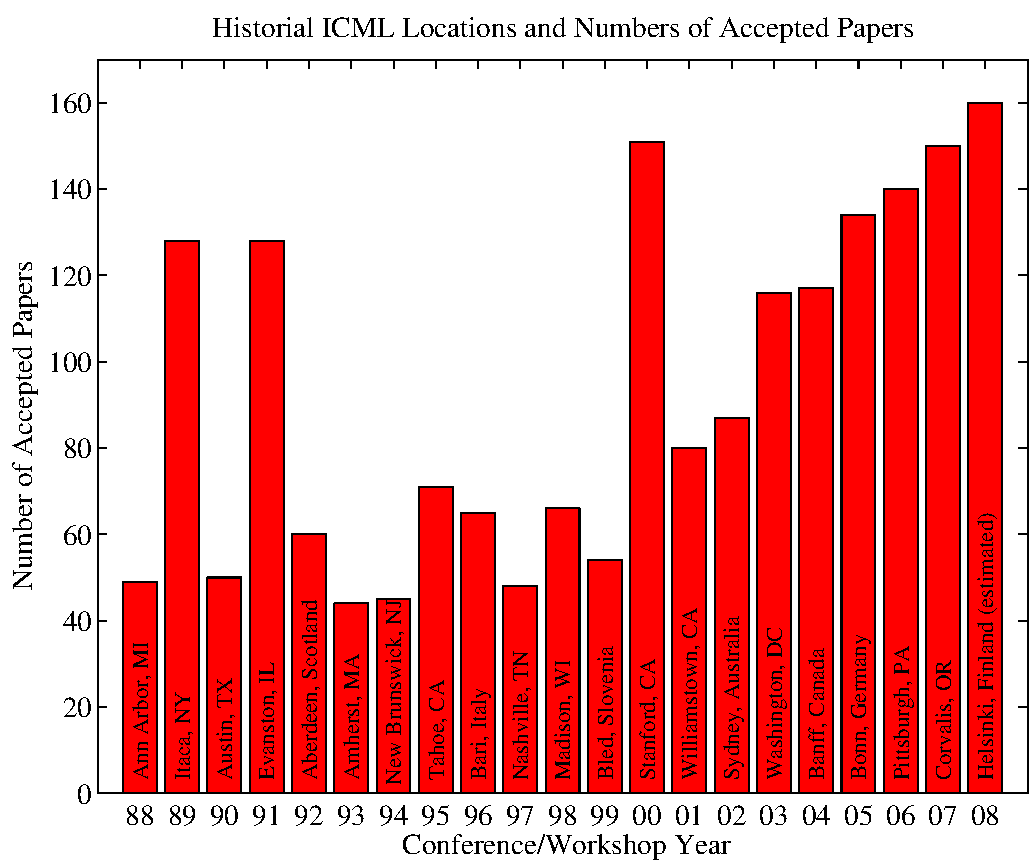
\includegraphics[width=\columnwidth]{icml_numpapers}}
\caption{Historical locations and number of accepted papers for International
  Machine Learning Conferences (ICML 1993 -- ICML 2008) and
  International Workshops on Machine Learning (ML 1988 -- ML
  1992). At the time this figure was produced, the number of
  accepted papers for ICML 2008 was unknown and instead estimated.}
\label{icml-historical}
\end{center}
\vskip -0.2in
\end{figure} 

\subsection{Figures}
 
You may want to include figures in the paper to help readers visualize
your approach and your results. Such artwork should be centered,
legible, and separated from the text. Lines should be dark and at
least 0.5~points thick for purposes of reproduction, and text should
not appear on a gray background.

Label all distinct components of each figure. If the figure takes the
form of a graph, then give a name for each axis and include a legend
that briefly describes each curve. Do not include a title inside the
figure; instead, the caption should serve this function.

Number figures sequentially, placing the figure number and caption
{\it after\/} the graphics, with at least 0.1~inches of space before
the caption and 0.1~inches after it, as in
Figure~\ref{icml-historical}.  The figure caption should be set in
9~point type and centered unless it runs two or more lines, in which
case it should be flush left.  You may float figures to the top or
bottom of a column, and you may set wide figures across both columns
(use the environment {\tt figure*} in \LaTeX), but always place
two-column figures at the top or bottom of the page.

\subsection{Algorithms}

If you are using \LaTeX, please use the ``algorithm'' and ``algorithmic'' 
environments to format pseudocode. These require 
the corresponding stylefiles, algorithm.sty and 
algorithmic.sty, which are supplied with this package. 
Algorithm~\ref{alg:example} shows an example. 

\begin{algorithm}[tb]
   \caption{Bubble Sort}
   \label{alg:example}
\begin{algorithmic}
   \STATE {\bfseries Input:} data $x_i$, size $m$
   \REPEAT
   \STATE Initialize $noChange = true$.
   \FOR{$i=1$ {\bfseries to} $m-1$}
   \IF{$x_i > x_{i+1}$} 
   \STATE Swap $x_i$ and $x_{i+1}$
   \STATE $noChange = false$
   \ENDIF
   \ENDFOR
   \UNTIL{$noChange$ is $true$}
\end{algorithmic}
\end{algorithm}
 
\subsection{Tables} 
 
You may also want to include tables that summarize material. Like 
figures, these should be centered, legible, and numbered consecutively. 
However, place the title {\it above\/} the table with at least 
0.1~inches of space before the title and the same after it, as in 
Table~\ref{sample-table}. The table title should be set in 9~point 
type and centered unless it runs two or more lines, in which case it
should be flush left.

% Note use of \abovespace and \belowspace to get reasonable spacing 
% above and below tabular lines. 

\begin{table}[t]
\caption{Classification accuracies for naive Bayes and flexible 
Bayes on various data sets.}
\label{sample-table}
\vskip 0.15in
\begin{center}
\begin{small}
\begin{sc}
\begin{tabular}{lcccr}
\hline
\abovespace\belowspace
Data set & Naive & Flexible & Better? \\
\hline
\abovespace
Breast    & 95.9$\pm$ 0.2& 96.7$\pm$ 0.2& $\surd$ \\
Cleveland & 83.3$\pm$ 0.6& 80.0$\pm$ 0.6& $\times$\\
Glass2    & 61.9$\pm$ 1.4& 83.8$\pm$ 0.7& $\surd$ \\
Credit    & 74.8$\pm$ 0.5& 78.3$\pm$ 0.6&         \\
Horse     & 73.3$\pm$ 0.9& 69.7$\pm$ 1.0& $\times$\\
Meta      & 67.1$\pm$ 0.6& 76.5$\pm$ 0.5& $\surd$ \\
Pima      & 75.1$\pm$ 0.6& 73.9$\pm$ 0.5&         \\
\belowspace
Vehicle   & 44.9$\pm$ 0.6& 61.5$\pm$ 0.4& $\surd$ \\
\hline
\end{tabular}
\end{sc}
\end{small}
\end{center}
\vskip -0.1in
\end{table}

Tables contain textual material that can be typeset, as contrasted 
with figures, which contain graphical material that must be drawn. 
Specify the contents of each row and column in the table's topmost
row. Again, you may float tables to a column's top or bottom, and set
wide tables across both columns, but place two-column tables at the
top or bottom of the page.
 
\subsection{Citations and References} 

Please use APA reference format regardless of your formatter
or word processor. If you rely on the \LaTeX\/ bibliographic 
facility, use {\tt natbib.sty} and {\tt icml2017.bst} 
included in the style-file package to obtain this format.

Citations within the text should include the authors' last names and
year. If the authors' names are included in the sentence, place only
the year in parentheses, for example when referencing Arthur Samuel's
pioneering work \yrcite{Samuel59}. Otherwise place the entire
reference in parentheses with the authors and year separated by a
comma \cite{Samuel59}. List multiple references separated by
semicolons \cite{kearns89,Samuel59,mitchell80}. Use the `et~al.'
construct only for citations with three or more authors or after
listing all authors to a publication in an earlier reference \cite{MachineLearningI}.

Authors should cite their own work in the third person
in the initial version of their paper submitted for blind review.
Please refer to Section~\ref{author info} for detailed instructions on how to
cite your own papers.

Use an unnumbered first-level section heading for the references, and 
use a hanging indent style, with the first line of the reference flush
against the left margin and subsequent lines indented by 10 points. 
The references at the end of this document give examples for journal
articles \cite{Samuel59}, conference publications \cite{langley00}, book chapters \cite{Newell81}, books \cite{DudaHart2nd}, edited volumes \cite{MachineLearningI}, 
technical reports \cite{mitchell80}, and dissertations \cite{kearns89}. 

Alphabetize references by the surnames of the first authors, with
single author entries preceding multiple author entries. Order
references for the same authors by year of publication, with the
earliest first. Make sure that each reference includes all relevant
information (e.g., page numbers).

\subsection{Software and Data}

We strongly encourage the publication of software and data with the
camera-ready version of the paper whenever appropriate.  This can be
done by including a URL in the camera-ready copy.  However, do not
include URLs that reveal your institution or identity in your
submission for review.  Instead, provide an anonymous URL or upload
the material as ``Supplementary Material'' into the CMT reviewing
system.  Note that reviewers are not required to look a this material
when writing their review.

% Acknowledgements should only appear in the accepted version. 
\section*{Acknowledgements} 
 
\textbf{Do not} include acknowledgements in the initial version of
the paper submitted for blind review.

If a paper is accepted, the final camera-ready version can (and
probably should) include acknowledgements. In this case, please
place such acknowledgements in an unnumbered section at the
end of the paper. Typically, this will include thanks to reviewers
who gave useful comments, to colleagues who contributed to the ideas, 
and to funding agencies and corporate sponsors that provided financial 
support.  


% In the unusual situation where you want a paper to appear in the
% references without citing it in the main text, use \nocite
\nocite{langley00}

\bibliography{example_paper}
\bibliographystyle{icml2017}

\end{document} 


% This document was modified from the file originally made available by
% Pat Langley and Andrea Danyluk for ICML-2K. This version was
% created by Lise Getoor and Tobias Scheffer, it was slightly modified  
% from the 2010 version by Thorsten Joachims & Johannes Fuernkranz, 
% slightly modified from the 2009 version by Kiri Wagstaff and 
% Sam Roweis's 2008 version, which is slightly modified from 
% Prasad Tadepalli's 2007 version which is a lightly 
% changed version of the previous year's version by Andrew Moore, 
% which was in turn edited from those of Kristian Kersting and 
% Codrina Lauth. Alex Smola contributed to the algorithmic style files.  
